
\subsection{研究目标}
% 武旭同话术,待修改
基于上述研究进展,本研究面向社会-水文学研究前沿,以黄河流域为研究区,结合水文气象观测、社会经济统计、历史数据重建、遥感反演等获取多源数据,借助统计分析和模型模拟等手段,分析黄河流域人水关系的演变过程和驱动机制。具体研究目标如下:

(1)发展识别人水关系演变规律的分析框架,分别在历史时期和现代治黄时期,揭示了黄河流域人水关系演变过程、分析了不同阶段驱动流域人水关系演变的主要原因。

(2)发展流域人水关系演变机制分析的因果推断方法,建立黄河流域社会-生态系统的多主体模型,识别推动人水关系变化的关键机制,定量评估其产生的影响。


\subsection{研究内容}

本研究具体包含以下主要内容:

% 开题报告
(1)黄河流域历史时期流域水沙特征演变:识别历史时期不断增强的人类活动压力超越气候周期变化的驱动力的时间,以及两者主导并推动黄河流域水沙特征突破临界点的稳态转换过程,分析该稳态转换发生之前黄河的人水关系状态。
% 接下来利用建立的分析框架对黄河流域历史上的大事记进行分析,梳理出黄河流域人-水关系演变的主要脉络。最后利用系统回顾法,整合近代有研究以来对黄河人-水关系变化的定量分析成果,建立黄河流域人-水关系变化数据库,综合分析有研究以来人-水系统的主要驱动因素及演化路径。 

(2)现代治黄时期黄河流域的水治理演变:现代治黄的主要特征是强调流域系统综合治理,本研究分析上世纪六十年代以来黄河流域“有多少水、怎么用水、怎么分水”如何随时间变化,以及三者如何共同体现流域水治理变化,并解释这些变化背后流域系统如何被人类活动所主导。

(3)黄河流域分水制度变化的影响:在识别黄河流域现代水治理转变过程的基础上,分析治理转变期间,1987年和1998年两次流域水资源分配制度变化对流域系统的驱动机制,及其对社会-生态系统结构自上而下的重塑,定量识别该制度变化对流域不同地区用水的影响。

(4)黄河灌溉水分配的多主体建模:针对同样的制度变化过程,发展黄河流域粮食灌溉响应分水制度的多主体模型,模拟利益相关者对流域系统环境和制度变化的响应机制。自下而上分析粮食灌溉用水者对黄河流域水资源分配制度变化的适应过程,解析其用水来源对变化的响应。

基于上述研究内容,本研究的技术路线如图\ref{ch1:fig:workflow}所示:

\begin{figure}[htb] % use float package if you want it here
    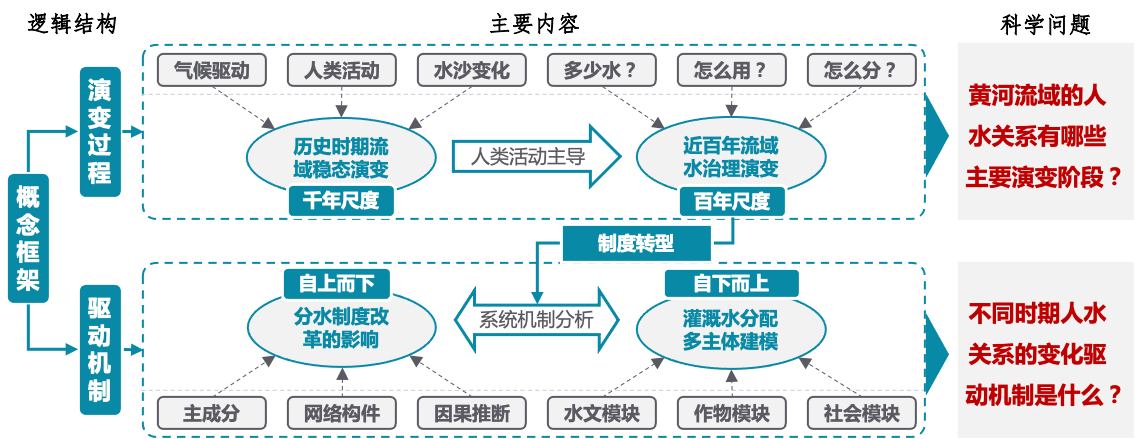
\includegraphics[width=\textwidth]{img/ch1/ch1_workflow.png}
    \caption{研究技术路线图}\label{ch1:fig:workflow}
\end{figure}

首先,针对历史时期和现代治黄的特点分别发展发展流域系统人水关系演变的识别框架,厘定怎样的变化可以被识别为发生了“流域人水关系演变”,以及有哪些潜在的驱动机制会导致这些变化,并总结黄河流域人水关系的演变过程:
(1)人类主导流域水沙特征变化是黄河人水关系变化的关键标志,黄河流域的水沙特征在历史时期发生从气候周期驱动向人类活动主导的过程。本研究使用历史重建资料和数据变化趋势识别病分析这一变化过程。
(2)水治理是现代流域人水关系变化的主要驱动力,黄河流域的“自然-社会二元水循环”在现代治黄时期则已由人类活动主导,使用综合指标构建和断点识别来识别流域水治理系统发生稳态转换的过程。
通过整合历史时期和人民治黄时期的人水关系演变,可以回答“黄河流域的人水关系有哪些主要演变阶段?”的科学问题,并总结各阶段黄河流域人水关系的特征。

针对现代治黄时期流域治理转变由人类制度主导的特点,接下来的两章以制度变化为落脚点,以对黄河流域影响最为深远的水资源分配制度为例,分别从自上而下和自下而上两个路径分析流域人水关系变化的驱动机制:
(1)自上而下:使用主成分分析、社会-生态系统网络构件识别、因果推断模型,分析制度变化对黄河流域系统结构及不同地区用水量的影响。
(2)自下而上:使用由人类模块和自然模块耦合构成的多主体模型,分析农业用水决策者的如何响应环境和制度变化,改变其水资源利用的过程。

\subsection{关键科学问题}

(1)黄河流域的人水关系有哪些主要演变阶段?

(2)不同时期人水关系变化的驱动机制是什么?
